\documentclass[11pt]{article}
\usepackage[utf8]{inputenc}
\usepackage{fancyhdr}
\usepackage[margin=1.25cm]{geometry}

\title{COMP37111 - Advanced Computer Graphics Notes}
\author{Sam Littlefair}

\usepackage{listings}
\usepackage{todonotes}
\usepackage{natbib}
\usepackage{graphicx}
\graphicspath{ {./img/} }
\usepackage{hyperref}
\usepackage{enumerate}
\usepackage{xcolor}
\usepackage{mathtools}
\usepackage{empheq}
\usepackage[skins,theorems]{tcolorbox}
\usepackage{wrapfig}
\usepackage{minipage-marginpar}

\definecolor{myblue}{rgb}{.8, .7, 1}
\newcommand*\mybluebox[1]{%
\colorbox{myblue}{\hspace{1em}#1\hspace{1em}}}

\begin{document}

  \maketitle


  \section{Course Unit Structure}
  \begin{itemize}
    \item 10 credit module. Online exam 75\%.

    \item 30 hour individual lab marked out of 20, due Friday 7 Dec 2018.
    \begin{itemize}
      \item Design  and implement a simulation with particle systems.
      \item Model real-time behaviour of a particle system.
      \item Give analysis of performance, real-time interaction with varying number of particles.
    \end{itemize}
  \end{itemize}

  \begin{itemize}
    \item The course is split into 4 main sections, the first 2 by Toby Howard:
    \begin{enumerate}
      \item \textit{Generative Modelling:} Creating 3D models and textures from sets of rules. (Particle Systems, Fractals..)
      \item \textit{Modelling and model acquisition:} Where to get meshes. (Laser scanning, Triangulation..)
    \end{enumerate}

    \item And the last 2 by Steve Pettifer:
    \begin{enumerate}
      \setcounter{enumi}{2}
      \item \textit{Global illumination:} The rendering equation, ray tracing, luminosity..
      \item \textit{Real-time rendering:} Maximising performance (i.e. frame-rate) using methods like culling.
    \end{enumerate}
  \end{itemize}
  \subsection{Resources}
  \begin{itemize}
    \item Real-Time Rendering book. (Tomas Möller, Eric Haines, Naty Hoffman)
    \item \href{http://www.realtimerendering.com/}{Real-Time Rendering website.}
  \end{itemize}

  \section{Generative Modelling}
  For most things we can use polygons, but there are a lot of phenomena that are not fundamentally polygonal - Liquids, fire, smoke, trees, bushes, hair etc. For these we use generative (aka procedural) modelling techniques:
  \iffalse
  \begin{enumerate}
    \item Particle Systems.
    \item Fractals.
    \item Grammar based modelling.
  \end{enumerate}
  \fi

  \subsection{Particle Systems}
  Each particle has a set of properties which
  change over time:
  \begin{itemize}
    \item Size, shape, colour, opacity.
    \item Position, velocity, acceleration.
    \item Age, lifetime.
  \end{itemize}
  \newpage
  \subsubsection{Particle Attributes}
  For some property P of the particle, we compute its initial value using:\\
  \begin{empheq}[box=\mybluebox]{align}
    P_{initial} = P_{mean} + (Random() \times P_{variance} )
  \end{empheq}

  \subsubsection{Computing particle position}
  You can compute the position of a particle at time $t$ using standard equations of motion:\\

  \begin{empheq}[box=\mybluebox]{align}
    x_{p} &= v_{p}tcos\beta_{p}\\
    y_{p} &= v_{p}tsin\beta_{p}-\frac{1}{2}gt^{2}
  \end{empheq}
  \begin{itemize}
    \item $x_{p} =$ Particle Velocity in $m^{2}$
    \item $\beta_{p} =$ Particle Angle in degrees
    \item $g =$ Acceleration of Gravity in $ms^{2}$
    \item $t =$ Time in $s$
  \end{itemize}

  For particle bounces, check if $y = y_{ground}$, if so reset the particle position and dampen the velocity. Bounces are a special case of particle/polygon intersection, we need fast intersection algorithms.\\

  \todo[inline, color=green!40]{TODO: Add efficiency and scalability section here.}

  \subsubsection{Particle System Algorithm}
  For every frame:
  \begin{enumerate}
    \item Remove any particles past their lifetime.
    \item Create new particles and initialise them.
    \item Update attributes for each particle.
    \begin{itemize}
      \item Position:
      \begin{itemize}
        \item Detect collisions of particles with environment.
        \item Detect inter-particle collisions.
      \end{itemize}
      \item Colour, acceleration, etc.
    \end{itemize}

    \item Render current particles.
  \end{enumerate}
  \subsubsection{Particle System Algorithm}

  Particle systems engines are often
  driven by an external textual script which gives: Laws, initial values, limits, etc. The engine reads script, sets parameters, then executes rules.
  \newpage
  \subsubsection{Rendering Ideas - 1}
  Particles rendered simply as pixels/groups of pixels, raw or anti-aliased.\\
  \begin{center}
    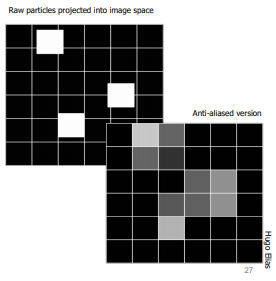
\includegraphics[scale=0.8]{render1}
  \end{center}
  \subsubsection{Rendering Ideas - 2}
  Connect old and new particles with a line segment.
  \begin{center}
    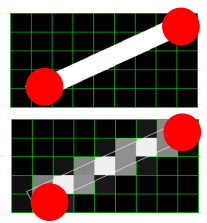
\includegraphics[scale=0.9]{render2}
  \end{center}

  \subsubsection{Rendering Ideas - 3}
  Particles rendered as Gaussian Kernals aka splats.
  \begin{center}
    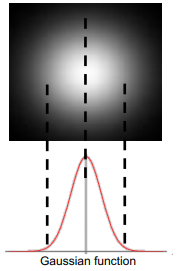
\includegraphics[scale=0.9]{render3}
  \end{center}

  \subsubsection{Rendering Ideas - 1}
  Particles rendered as small alpha-textured (partially transparent) quads. Like billboards, always aligned to screen.
  \begin{center}
    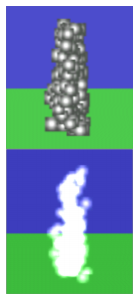
\includegraphics[scale=0.7]{render4}
  \end{center}

  \subsubsection{Rendering Grass}
  We can make the particles path draw the shape of the grass.


  \subsection{Fractal Modelling}
  A lot of natural things are \textbf{self-similar} meaning they have the same shape at different scales.

  \subsubsection{Modelling fractal curves}
  We can use \textbf{recursive subdivision}:
  \begin{itemize}
    \item Take mid-point of line, displace it randomly
    \item Replace first line with two new lines
    \item Repeat recursively until required level of detail.

  \end{itemize}
  \begin{center}
    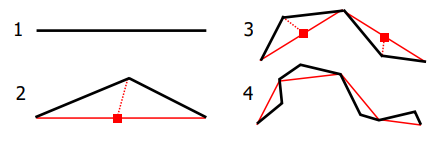
\includegraphics{recursive_subdivision}
  \end{center}

  \subsubsection{3D terrain generation}

  \lstset{language=Java}

  \begin{lstlisting}
    splitPoly (vertices) {
    if (!detailedEnough (vertices) ) {
    splitPoints = computeSplitPoints(vertices)
    foreach splitPoints as s {
    splitPoly (s);
    }
    }
    }
  \end{lstlisting}
  \newpage
  \subsection{Grammar-based modelling}
  We can define objects using simple grammar
  production rules, trace out path using commands like:\\

  \begin{minipage}[c]{0.45\textwidth}
    \begin{itemize}
      \item F = move 1 unit forwards
      \item L = turn left through angle $\theta$
      \item R = turn right through angle $\theta$
    \end{itemize}
  \end{minipage}
  \hfill
  \begin{minipage}[c]{0.55\textwidth}
    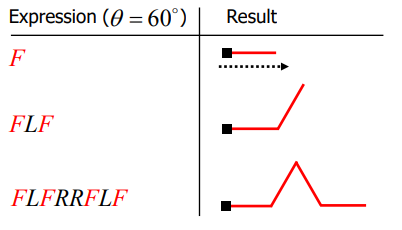
\includegraphics[scale=0.7]{grammar_based}

  \end{minipage}

  We can apply rules recursively, for example:\\

  \begin{center}
    $\textcolor{red}{F} \xrightarrow{} \textcolor{red}{F}L\textcolor{red}{F}RR\textcolor{red}{F}L\textcolor{red}{F}$
  \end{center}

  \subsection{L-Systems}
  L-systems add \textbf{push} and \textbf{[pop]} commands, which
  permit more complex structures:\\

  \begin{minipage}[c]{0.5\textwidth}
    \begin{center}
      $\textcolor{red}{F} \xrightarrow{} \textcolor{red}{F}\textbf{[R\textcolor{red}{F}]}\textcolor{red}{F}\textbf{[L\textcolor{red}{F}]}\textcolor{red}{F}$
    \end{center}
  \end{minipage}
  \hfill
  \begin{minipage}[c]{0.5\textwidth}
    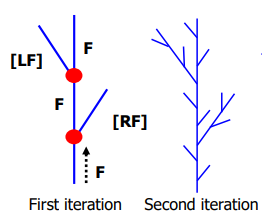
\includegraphics[scale=0.7]{lsystem}

  \end{minipage}
\end{document}
